\documentclass{article}
\usepackage[utf8]{inputenc}
\usepackage[spanish]{babel}

% Formato de página
\usepackage[letterpaper, margin = 1.5cm]{geometry}

% Más opciones para enumerar
\usepackage{enumitem}

% Manejo de imágenes
\usepackage{graphicx}
\usepackage{wrapfig}
\graphicspath{{img/}}
\usepackage{float}

\begin{document}
    \title{
        Fundamentos de bases de datos \\
        Tarea 3 \\
        Modelo Relacional
    }
    \author{
        Díaz Gómez Silvia \\
        Eugenio Aceves Narciso Isaac \\
        Quiroz Castañeda Edgar
    }
    \date {
        22 de marzo del 2019    
    }
    \maketitle

    \section{Preguntas de repaso}
    \begin{enumerate}[label = \alph*.]
        \item ¿Qué es una \textbf{relación} y qué características tiene?
        \item ¿Qué es un \textbf{esquema de relación}?
        \item ¿Qué es una \textbf{llave primaria} ¿qué es una \textbf{llave 
        candidata}? ¿qué es una \textbf{llave mínima}? ¿qué es una \textbf{super
        llave}
        \item ¿Qué restricciones impone una \textbf{llave primaria} y una llave 
        foránea al modelo de dato relacional?
        \item Investiga cómo se traducen las \textbf{categorías} (presentes en
        el \textbf{modelos E/R}) al \textbf{modelos relacional}. Proporciona un 
        ejemplo.
    \end{enumerate}

    \section{Modelo relacional}
    Traduce el siguiente modelo \textbf{Entidad/Relación} a su correspondiente 
    \textbf{Modelo Relacional}:
    
    \begin{center}
        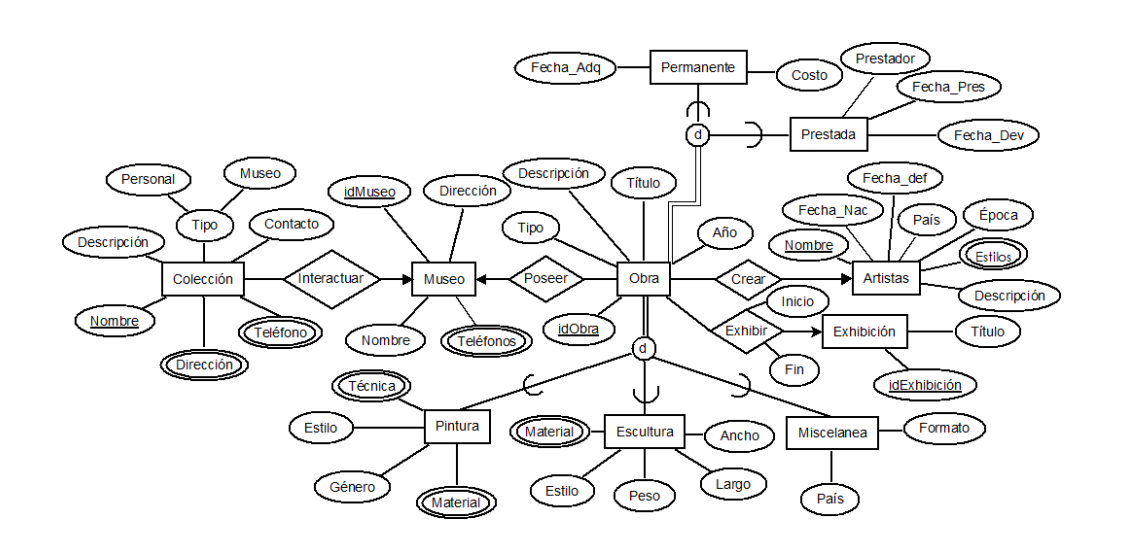
\includegraphics[width=1\textwidth]{er1.png}
    \end{center}

    \begin{figure}[H]
    	\begin{center}
    		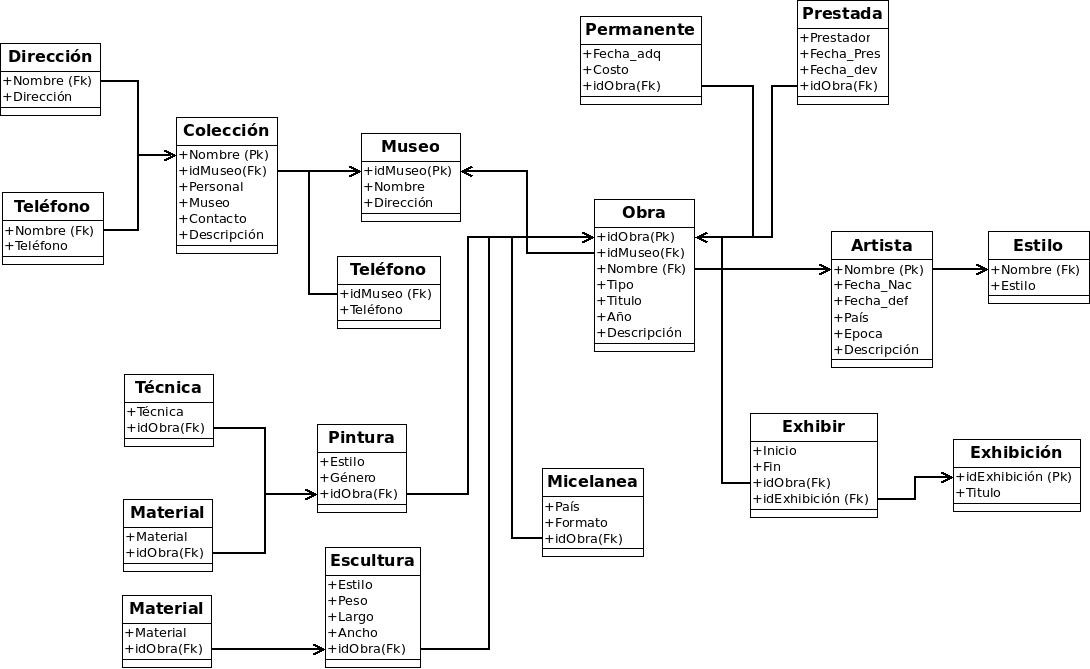
\includegraphics[width=1\textwidth]{MRProblema2.jpeg}
    	\end{center}
    	\caption{Traducción del modelo E-R de la figura anterior al modelo Relacional.}
    \end{figure}
        
    \section{Modelo relacional}
    Traduce s su correspondiente \textbf{Modelo Relacional} el problema del 
    \textbf{Sistema de Información Geográfica (Tarea 1)}. Se realizaste alguna
    modificación a tu diseño orignal (para mejorarlo) indica los cambios hechos 
    y la justificación de los mismos.\\
    En cualquier caso, deberás mostrar el \textbf{diagrama E/R} y su
    correspondiente traducción. Es importante que muetres tanto las 
    \textbf{restricciones de entidad} como las de \textbf{integridad referencial}.
    
    \begin{figure}[H]
    	\begin{center}
    		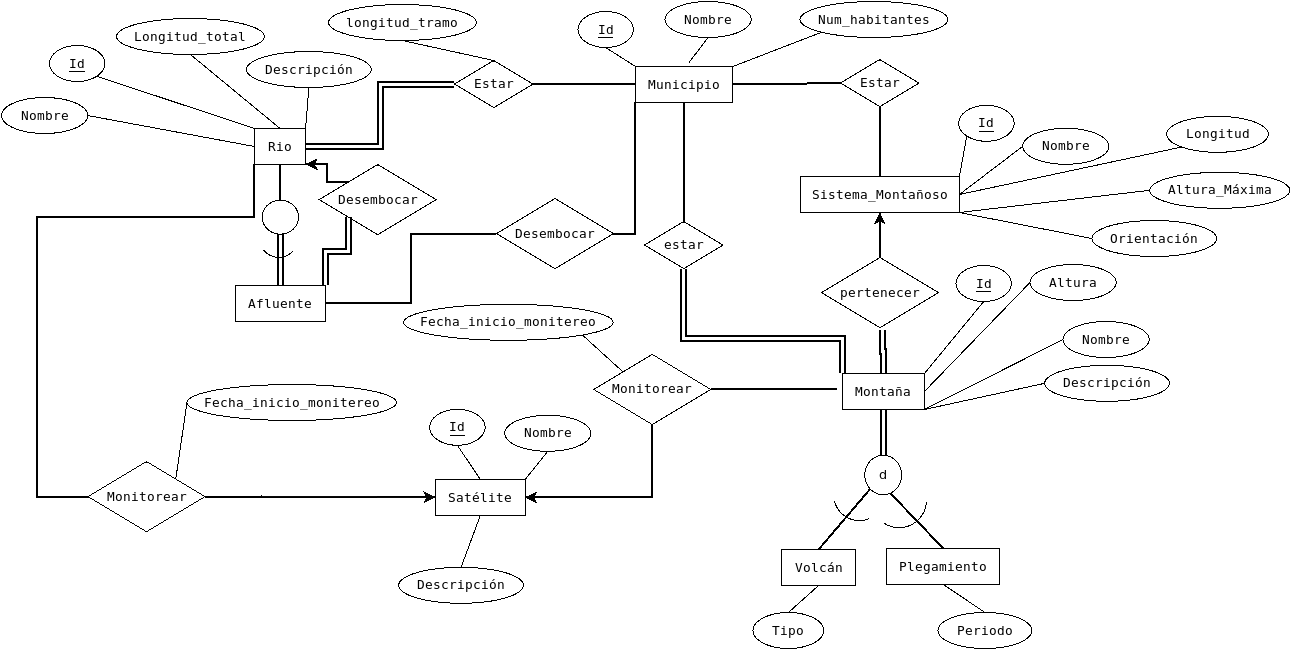
\includegraphics[width=1\textwidth]{2b.png}
    	\end{center}
    	\caption{Modelo E-R para el Sistema de Información Geográfica.}
    \end{figure}
    
    \begin{figure}[H]
      \begin{center}
      	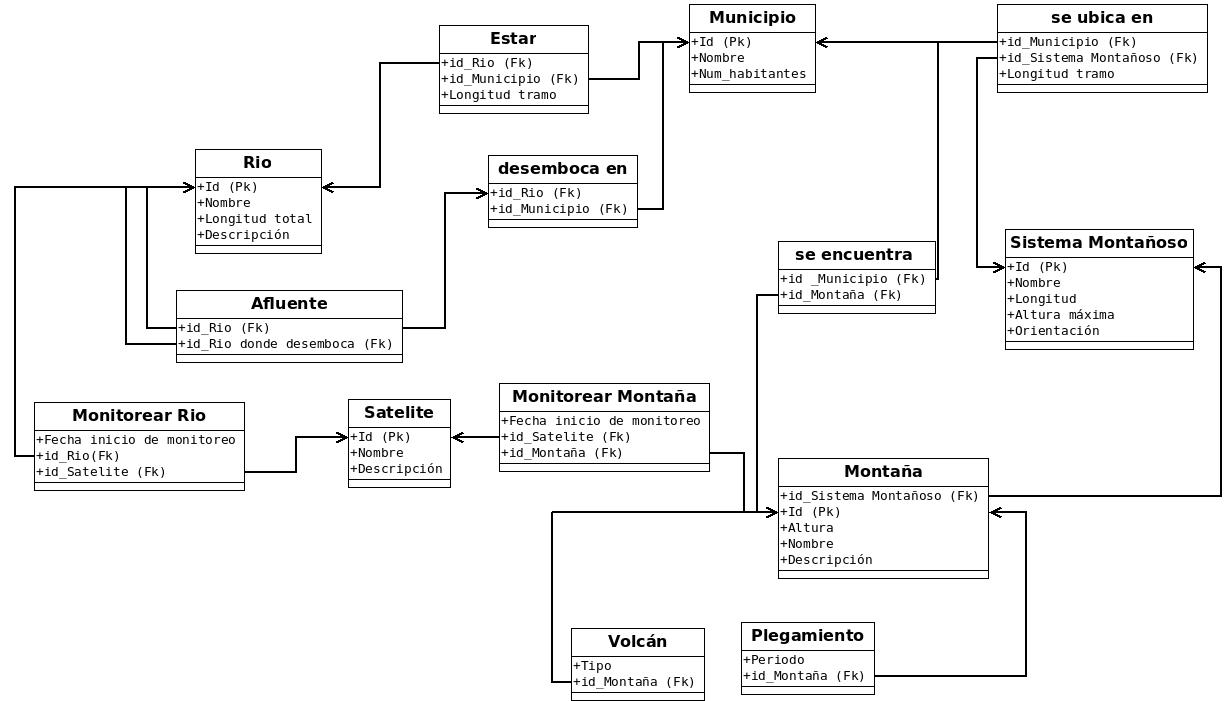
\includegraphics[width=1\textwidth]{esquemaRelacionalGeo.jpeg}
      \end{center}
      \caption{Traducción del modelo E-R para el Sistema de Información Geográfica a  Esquema Relacional.}
   \end{figure}

    \section{Lectura}
    Leer el artícula \textbf{Codd's 12 Rules for a RDBMS}. Explica con tus 
    propias palabras cada una de las 12 reglas de \textbf{Codd}.\\
    Indica por qué consideras que son importantes y si, hasta el momento de lo 
    comentado en el curso, sería posible que un \textbf{SMBD} pudiera cumplir 
    enteramente con lo que ahí se propone.
    
    \begin{itemize}
    	\item\textbf{Regla 1 : The Information Rule}\\
    	 Basicamente habla acerca de como se almacena la información y la forma en que se hace es a través una tabla.
    	\item\textbf{Regla 2 : Guaranteed Access Rule}\\
    	
    	En esta regla se menciona la importancia de un identificador o llave primaria, además de  que los datos sean atomicos ya que son de suma importancia para poder garantizar la accesibilidad a los datos.
    	
    	\item\textbf{Regla 3: Systematic Treatment of NULL Values}\\
    	
    	Esta regla hace referencia a los valores nulos, que no representan una cadena vacía o un cero sino que son valores desconocidos por lo tanto el RDBMS admitirá un caracter distinto para representar dichos valores nulos. Los valores nulos indican que no se tiene información de ese campo, además los nulos deben propagarse ante las operaciones matematicas y de cadenas, es decir si sumamos un valor nulo con algún elemento distinto de nulo el resultado sera un valor nulo.
    	
    	\item\textbf{Regla 4: Dynamic Online Catalog Based on the Relational Model}\\
    	Esta regla menciona que la base de datos debe ser autodescriptiva para poder por lo tanto permite utilizar 
    	
    	\item\textbf{Regla 5: Comprehensive Data Sublanguage Rule}\\
    	
    	\item\textbf{Regla 6: View Updating Rule}\\
    	
    	\item\textbf{Regla 7: High-Level Insert, Update, and Delete}\\
    	
    	\item\textbf{Regla 8: Physical Data Independence}\\
    	Esta regla menciona que a nivel fisico que es donde la base de datos almacena e implementa los metodos de acceso a los datos es independiente de la manera lógica en que se accede, por lo tanto los cambios que se hagan a nivel físico no le afecta al usuario puesto que al usuario no le interesa saber como se almacena o como se acceden a los datos. 
    	
    	\item\textbf{Regla 9: Logical Data Independence}\\
    	
    	\item\textbf{Regla 10: Integrity Independence}\\
    	
    	\item\textbf{Regla 11: Distribution Independence}\\
    	
    	\item\textbf{Regla 12: Non-Subversion Rule}\\
    	
    	
    \end{itemize}
\end{document}